\section{Source Selection}\label{sec:design:source}
We begin the algorithm with a list of $n$ sources in the plane. Each source has three parameters: $x$, $y$ and $z$. The $x$ and $y$ parameters define the spatial coordinates of the source while the z parameter is used to reflect the intensity of the source.
\\
\\
The sources are read in and are used to generate the Voronoi centres. Each centre has the following attributes:
\begin{enumerate}
\item An $x$, $y$, and $z$ value inherited from its source.
\item A Boolean value to determine if it is the circumcentre which defaults to false.
\item A centre clockwise to it if it lies on the convex hull which defaults to none.
\item A centre counter-clockwise to it if it lies on the convex hull which defaults to none.
\item A list of all its neighbouring points and the line that bisects them set into a tuple; the list is set to none by default.
\item A list of sources in the cell created by the centre which is set to none by default.
\item The cell's error which is set to zero by default as there are no sources at initialisation.
\item A list of all the cells that have been merged with this cell; by default, this is also set to none.
\end{enumerate} 
Sources are chosen as centres for a Voronoi cell if they have an intensity greater than some predetermined threshold. Once the set of centres, $C= \{c_0,c_1,...,c_n\}$, is created, it is sorted in lexical order i.e. by the $x$ values followed by the $y$ values if the $x$ values are equal. Once the centres have been created, generation of the Voronoi tessellation can begin.
\\
\\
For the sake of testing the system, the $x$ and $y$ coordinates of the sources were randomly generated on a $600 \times 600$ plane with the intensities, $z$, randomly generated as the absolute value of a random normal distribution, centred at zero with a standard deviation of $3000$. Using this, $10000$ sources were randomly generated. From these sources, we generated the centres to be used by the Voronoi, where these centres were sources with an intensity greater than one standard deviation of the mean. Since the absolute value of the source intensity was used, this includes all sources with an intensity greater than 3000, thus accounting for approximately $32\%$ of the sources.
\begin{figure}[H]
\centering
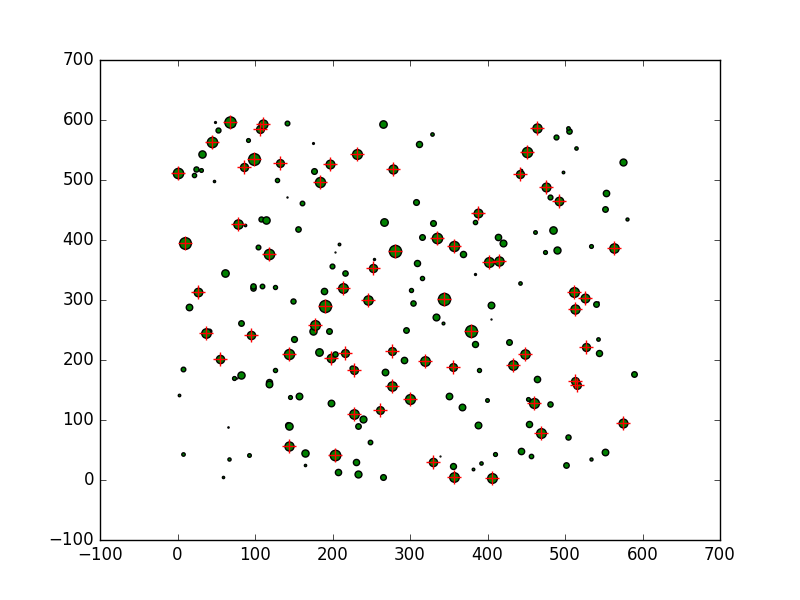
\includegraphics[width=0.8\textwidth]{Images/sources.png}
\caption{ All sources (green circles) with those selected as centres (red crosses).}
\label{fig:source}
\end{figure}
Figure \ref{fig:source} shows sources in green with their intensities represented by the size of the circle on the plane; for simplicity, only $200$ points were generated. The crosses in red represent the centres that were used to generate the Voronoi tessellation.
